\begin{Exercise}[title={栈},difficulty=1]
\label{ex:stack}
\Question \label{ex:stack q1} 创建一个固定大小保存整数的栈。
它无须超出限制的增长。定义~\func{push} 
函数——将数据放入栈,和~\func{pop} 
函数——从栈中取得内容。栈应当是后进先出(LIFO)的。

\begin{figure}[H]
\caption{一个简单的~LIFO 栈}
\label{fig:stack}
\begin{center}
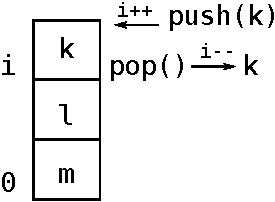
\includegraphics[scale=0.65]{fig/stack.pdf}
\end{center}
\end{figure}

\Question \label{ex:stack q2} 更进一步。编写一个~\func{String} 方法将栈转化为字符串形式的表达。
可以这样的方式打印整个栈:
\lstinline{fmt.Printf("My stack %v\n", stack)}

\noindent{}栈可以被输出成这样的形式:
\texttt{[0:m] [1:l] [2:k]}

\end{Exercise}

\begin{Answer}

\Question 
%%\subsection*{Define our type} maybe nice to do this
首先定义一个新的类型来表达栈;需要一个数组(来保存键)和一个指向最后一个元素的索引。
这个小栈只能保存~10 个元素。

\begin{lstlisting}
type stack struct { |\coderemark{\emph{栈}不应该被导出}|
    i    int 
    data [10]int  
}
\end{lstlisting}

然后需要~\func{push} 和~\func{pop} 函数来使用这个。
\emph{首先展示一下\emph{错误}{}的解法!}
在~Go 的数据传递中,是\emph{值传递},意味着一个副本被创建并传递给函数。
\func{push} 函数的第一个版本大约是这样:

\begin{lstlisting}
func (s stack) push(k int) { |\coderemark{工作于参数的副本}|
	if s.i+1 > 9 {
		return
	}
	s.data[s.i] = k
	s.i++
}
\end{lstlisting}
函数对~\type{stack} 类型的变量~\var{s} 进行处理。
调用这个,只需要~\lstinline{s.push(50)},将整数 50 放入栈中。
但是 push 函数得到的是~\var{s} 的副本,所以它\emph{不会}有\emph{真正}的结果。
用这个方法,不会有内容放入栈中,例如下面的代码:

\begin{lstlisting}
var s stack |\coderemark{让~\var{s} 是一个~\type{stack} 变量}|
s.push(25)
fmt.Printf("stack %v\n", s);
s.push(14)
fmt.Printf("stack %v\n", s);
\end{lstlisting}
打印:
\vskip\baselineskip
\begin{display}
stack [0:0]
stack [0:0]
\end{display}
\vskip\baselineskip

为了解决这个,需要向函数~\func{push} 提供一个指向栈的指针。
这意味着需要修改~\func{push} 

\lstinline{func (s stack) push(k int)} 
$\rightarrow$
\lstinline{func (s *stack) push(k int)}

应当使用~\func{new()}(参阅第~\ref{chap:beyond} 章``\titleref{sec:allocation with new}''小节)
创建\emph{指针}指向的~\type{stack} 的空间,因此例子中的第~1 行需要是
\lstinline{s := new(stack)}

\noindent{}而两个函数变为:
\begin{lstlisting}
func (s *stack) push(k int) {
	s.data[s.i] = k
	s.i++
}

func (s *stack) pop() int {
	s.i--
	return s.data[s.i]
}
\end{lstlisting}
像下面这样使用
\begin{lstlisting}
func main() {
	var s stack
	s.push(25)
	s.push(14)
	fmt.Printf("stack %v\n", s)
}
\end{lstlisting}

\Question 这里有一个额外的问题,对于这个练习中编写打印栈的代码的时候非常有价值。
根据~Go 文档~\lstinline{fmt.Printf("\%v")} 可以打印实现了~\func{Stringer} 接口的任何值(\%v)。
为了使其工作,需要为类型定义一个~\func{String()} 函数:
\begin{lstlisting}[caption=stack.String()]
func (s stack) String() string {
	var str string
	for i := 0; i <= s.i; i++ {
		str = str + "[" +
			strconv.Itoa(i) + ":" + strconv.Itoa(s.data[i]) + "]"
	}
	return str
}
\end{lstlisting}
\end{Answer}
